\section{The differential on the Morse complex} \label{section:morse_differential}

Continuing with the program sketched in Section \ref{section:morse_complex}, we are to define a differential on the Morse complex using a pseudogradient adapted to our Morse function $f$ and satisfying the Palais-Smale property, as explained in Section \ref{section:pseudogradients}. More precisely, we are going to use the flow of our pseudogradient to define the differential, and then to prove that $\partial^2 = 0$.

\subsection{Definition of the differential}

Let $f$ a Morse function, and $X$ a pseudogradient adapted to it and satisfying the Smale condition. Then, we can define for each pair of critical points $a, b \in \crit(f)$, the manifold $\mathcal{L}(a,b)$. Recall that, when $\text{Ind}(a) \leq \text{Ind}(b)$, this manifold is empty. Moreover, if $\text{Ind}(a) = \text{Ind}(b) + 1$, it is discrete. This is because
\[\text{dim} \mathcal{L}(a,b) = \text{Ind}(a) - \text{Ind}(b) - 1 .\]
In this Section we are going to show that, in fact, $\mathcal{L}(a,b)$ must be finite when $\text{Ind}(a) = \text{Ind}(b) + 1$, so it makes sense to define
\[n_X(a,b) := \# \mathcal{L}(a,b) \quad (\text{mod } 2),\]
which denotes the number of trajectories of the flow of $X$ which go from $a$ to $b$ (in infinite time). We are taking it modulo $2$ because our homology groups are defined over $\Z_2$. It is posible to define the Morse homology over $\Z$ also, but then orientations must be introduced. To keep it simple, we restrict ourselves to the case with $\Z_2$.

\begin{deff}
The {\bf differential of the Morse complex} with function $f$ and pseudogradient $X$ can be defined over the generators of $C_k(M,f,X)$ (this means, $a \in \crit_k(f)$) as
\begin{displaymath}
\partial_X (a) = \sum_{b \in \crit_{k-1}(f)} n_X(a,b) b .
\end{displaymath}
\end{deff}

Our aim in this Section will be to prove that it is well defined (this means, that $n_X(a,b)$ is well defined), and to show that $\partial_X^2 = 0$. To do that, we will need to study the space of broken trajectories.

\subsection{The space of broken trajectories. Compactness}

Consider $a, b \in \crit(f)$ with $\text{Ind}(a) > \text{Ind}(b)$. We already know that $\mathcal{L}(a,b)$ (the space of the trajectories from $a$ to $b$) is a smooth manifold. However, we are interested in study its compactification, in one hand to prove that $n_X(a,b)$ is well defined, and on the other hand to prove that $\partial_x^2 = 0$.

Instead of studying how to compactify the space $\mathcal{L}(a,b)$, we will introduce a candidate of its compactification, the space of broken trajectories, containing $\mathcal{L}(a,b)$. Then, we will define a meaningful topology on this space. Finally, we are going to show that this topology makes this space compact.

\begin{deff}
The {\bf space of broken trajectories} from $a$ to $b$ is the disjoint union
\[\overline{\mathcal{L}}(a,b) := \bigcup_{c_1,...,c_{m-1} \in \crit(f)} \mathcal{L}(a,c_1) \times \cdots \times \mathcal{L}(c_{m-1},b) ,\]
where the union spans all the tuples of critical points, regardless of the size of the tuple. In particular, $\mathcal{L}(a,b) \subset \overline{\mathcal{L}}(a,b)$.

It is important to notice that the only tuples of critical points contributing to the union are the ones such that $\text{Ind}(a) > \text{Ind}(c_1) > ... > \text{Ind}(c_{m-1}) > \text{Ind}(b)$.
\end{deff}

\begin{rmrk}
When $\text{Ind}(a) - \text{Ind}(b) = 1$, we have that $\overline{\mathcal{L}}(a,b) = \mathcal{L}(a,b)$.
\end{rmrk}

\begin{rmrk}
Suppose that $\text{Ind}(a) - \text{Ind}(b) = 2$, and take $k = \text{Ind}(a)$. Then,
\[\overline{\mathcal{L}}(a,b) = \mathcal{L}(a,b) \bigcup \left[ \bigcup_{c \in \crit_{k-1}} \mathcal{L}(a,c) \times \mathcal(c,b) \right] .\]
We can see that in the union above, the dimension of $\mathcal{L}(a,b)$ is $1$, whereas $\text{dim} \mathcal{L}(a,c) = \text{dim} \mathcal{L}(c,b) = 0$ for all $c \in \crit_{k-1}(f)$. Thus, we are adding some points to a 1-dimensional manifold.
\end{rmrk}

With this definition, we can introduce a topology on the space of broken trajectories.

For each $p \in \crit(f)$, let $\Omega(p) \subset M$ denote the domain of the Morse chart centered in $p$. If necessary, shrink some of these domains to guarantee that $\Omega(p) \cap \Omega(q) = \emptyset$ for each pair $p \neq q \in \crit(f)$.

Let $\lambda \in \overline{\mathcal{L}}(a,b)$. Then, $\lambda = (\lambda_1,...,\lambda_m)$ for some trajectories $\lambda_i$. Consider $a = c_0, c_1, ..., c_{m-1}, c_m = b$ the critical points connected by these trajectories. Let $U_{i-1}^{-}$ be a neighbourhood of the exit point of $\lambda_i$ from the set $\Omega(c_{i-1})$ taken to lie in a level set of $f$. Similarly, take $U_i^+$ a neighbourhood of the entry point of $\lambda_i$ into the set $\Omega(c_i)$, also lying in a level set of $f$. Then, we have a family of sets, which we will denote by
\[\mathcal{W}(\lambda; U_0^{-}, U_1^{\pm},...,U_{m-1}^{\pm},U_m^{+}) .\]
Thus, we get a set of families, spanning all the broken trajectories $\lambda \in \overline{\mathcal{L}}(a,b)$ and the neighbourhoods $U_i^{\pm}$ that we just described. With all of this, we can define a topology on $\overline{\mathcal{L}}(a,b)$:

\begin{deff}
We say that a broken trajectory $\mu = (\mu_1,...,\mu_k)$ {\bf belongs} to a open neighbourhood $\mathcal{W}(\lambda,\mathbf{U})$ and denote it by $\mu \in \mathcal{W}(\lambda, \mathbf{U})$, if there are $0 < i_0 < ... < i_{k-1} < i_k = m$ such that

\begin{itemize}
	\item $\mu_j \in \mathcal{L}(c_{i_j},c_{i_{j+1}}) \ \forall j < k$.
	\item For all $j$, $\mu_j$ exits the chart $\Omega(c_{i_j-1})$ through some point in the interior of $U_{i_j-1}^{-}$, and enters the chart $\Omega(c_{i_j})$ through some point in the interior of $U_{i_j}^+$.
\end{itemize}

This way, the $\mathcal{W}(\lambda,\mathbf{U})$ form a fundamental system of open neighbourhoods to define the topology of $\overline{\mathcal{L}}(a,b)$.
\end{deff}

\begin{rmrk}
We can see that $\mu \in \mathcal{W}(\lambda, \mathbf{U})$ implies that $k \leq m$, this means, $\mu$ has less or equal components than $\lambda$. Equivalently, $\mu$ passes through the same number of critical points that $\lambda$ or less.
\end{rmrk}

This topology establishes that a broken trajectory $\mu$ is “close” to $\lambda$ if all the critical points connected by $\mu$ are also connected by $\lambda$ and if $\mu$ leaves $\Omega(c_{i_j})$ and enters $\Omega(c_{i_{j+1}})$ sufficiently close to $\lambda$.

\begin{rmrk}
This topology coincides with the topology of $\mathcal{L}(a,b)$ as a manifold.
\end{rmrk}

Finally, we can prove the central theorem of this Section:

\begin{theo}
The space $\overline{\mathcal{L}}(a,b)$ is compact.
\end{theo}

\begin{proof}
We will prove that $\overline{\mathcal{L}}(a,b)$ is sequentially compact, this means, that for any sequence $(l_n)_n$ we can extract a subsequence that is convergent to some $l \in \overline{\mathcal{L}}(a,b)$.

First of all, let $(l_n)_n \subset \mathcal{L}(a,b)$. The general case will follow from this one.

Let $l_n^{-}$ denote the exit point of the trajectory $l_n$ from $\Omega(a)$. As $l_n^- \in \partial \Omega(a)$, which is compact, we can extract a subsequence such that $l_{n_k}^- \xrightarrow[k \rightarrow \infty]{} a^-$, with $a^- \in \partial \Omega(a)$ and $a^- \in W^u(a)$.

Let $\gamma(t) = \varphi^t_X(a^-)$ be the trajectory of $X$ through $a^-$. By Proposition \ref{prop:connect_critical_points}, $c_1 = \displaystyle\lim_{t \rightarrow +\infty} \gamma(t)$ is a critical point, and $\gamma \in \mathcal{L}(a,c_1)$. Let $d^+$ denote the entry point of $\gamma$ into $\Omega(c_1)$. By the theorem of dependence of solutions of differential equations on the initial conditions, $l_n$ must also (at least for $n$ large enough) enter $\Omega(c_1)$ through a point $d_n^+$. We have that $\displaystyle\lim_{n \rightarrow \infty} d_n^+ = d^+$ by the following lemma:

\begin{lema} \label{morse_sequences}
Let $x \in M \backslash \crit(f)$, and $(x_n)_n$ a sequence that tends to $x$. Let $y_n$ a sequence of points such that $y_n$ and $x_n$ belong to the same trajectory of $X$ for each $n$, and $y$ belonging to the same trajectory as $x$. Moreover, suppose that $f(y_n) = f(y)$. Then,
\[\lim_{n \rightarrow \infty} y_n = y .\]
\begin{figure}[h] \label{figure:morse_sequences}
	\centering
	%Figure to illustrate the lemma 1.41
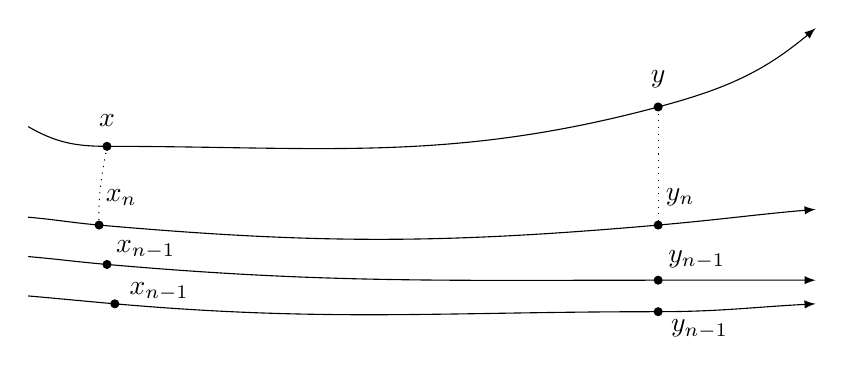
\begin{tikzpicture}
	\draw [arrows={-latex}] (0,2.75) to [out=330,in=180] (1,2.5)
to [out=0,in=195] (8,3) to [out=15,in=220] (10,4) ;
	\draw [fill] (1,2.5) circle [radius=0.05]
	node [label={[above]$x$}] {};
	\draw [fill] (8,3) circle [radius=0.05]
	node [label={[above]$y$}] {};

	\draw [arrows={-latex}] (0,1.6) to [out=355,in=175] (0.9,1.5) to [out=355,in=185] (8,1.5) to [out=5,in=185] (10,1.7);
	\draw [fill] (0.9,1.5) circle [radius=0.05]
	node [label={[above,xshift=8]$x_n$}] {};
	\draw [fill] (8,1.5) circle [radius=0.05]
	node [label={[above,xshift=8]$y_n$}] {};

	\draw [dotted] (1,2.5) to [out=260,in=92] (0.9,1.5);
	\draw [dotted] (8,3) to (8,1.5);

	\draw [arrows={-latex}] (0,1.1) to [out=355,in=175] (1,1) to [out=355,in=180] (8,0.8) to [out=0,in=180] (10,0.8);
	\draw [fill] (1,1) circle [radius=0.05]
	node [label={[above,yshift=-5,xshift=14]$x_{n-1}$}] {};
	\draw [fill] (8,0.8) circle [radius=0.05]
	node [label={[above,yshift=-3,xshift=14]$y_{n-1}$}] {};

	\draw [arrows={-latex}] (0,0.6) to [out=355,in=175] (1.1,0.5) to [out=355,in=180] (8,0.4) to [out=0,in=183] (10,0.5);
	\draw [fill] (1.1,0.5) circle [radius=0.05]
	node [label={[above,yshift=-6,xshift=16]$x_{n-1}$}] {};
	\draw [fill] (8,0.4) circle [radius=0.05]
	node [label={[below,xshift=15,yshift=-3]$y_{n-1}$}] {};
\end{tikzpicture}
	\caption{Illustration of Lemma \ref{morse_sequences}.}
\end{figure}
\end{lema}

\begin{proof}
Consider $U$ an open subset of $M \backslash \crit(f)$ such that it contains $x,y, x_n$ and $y_n$ (at least for $n$ sufficiently large). On $U$ we can define the vector field
\[Y = - \frac1{d f(X)} X .\]
Let $\psi^t$ be its flow. $Y$ and $X$ are colinear at each point, so they have the same trajectories. In addition,
\[f(\psi^t(z)) = f(z) - t .\]
Therefore, we can express $y_n$ as
\[y_n = \psi^{f(x_n)-f(y_n)}(x_n) = \psi^{f(x_n)-f(y)}(x_n) ,\]
and
\[y = \psi^{f(x)-f(y)}(x) .\]
So $\displaystyle\lim_{n \rightarrow \infty} y_n = y$.
\end{proof}

If $c_1 = b$ then $\displaystyle\lim_{n \rightarrow \infty} l_n = \gamma \in \mathcal{L}(a,b)$, so $(l_n)_n$ has a convergent subsequence. This means that we need to check what happens for $c_1 \neq b$.

The points $d_n^+$ do not belong to $W^s(c_1)$ (because, otherwise, we would have that $l_n \in \mathcal{L}(a,c_1)$, which contradicts our hypothesis). Therefore, $l_n$ exits $\Omega(c_1)$ through a point $d_n^-$. As before, we can extract a subsequence such that $\displaystyle\lim_{n \rightarrow \infty} d_n^- = d^-$.

We claim that $d^- \in W^u(c_1)$. Suppose that it is not the case. Let $\mu$ denote the trajectory of $X$ passing through $d^-$. If $d^- \notin W^u(c_1)$, there must be a point $d_{\ast}$ such that $f(d_{\ast}) = f(d_n^+)$. By the lemma that we just proved, $d_n^+ \xrightarrow[n \rightarrow \infty]{} d_{\ast}$, so $d_{\ast} = d^+$. Therefore, $d_{\ast} \in W^s(c_1)$. However, this is a contradiction, because $\mu$ passes through $d_{\ast}$ and exits $\Omega(c_1)$ through $d^-$. Therefore, we have proved that $d^- \in W^u(c_1)$.

If we repeat this process a finite number of times (as there is a finite number of critical points), we will be able to construct a subsequence $(l_n)_n$ and a broken trajectory $\lambda = (\lambda_1,...,\lambda_m)$ such that $\displaystyle\lim_{n \rightarrow \infty} l_n = \lambda$, as in Figure \ref{figure:limit_trajectories}.

\begin{figure}[h] \label{figure:limit_trajectories}
	\centering
	%Figure to illustrate the end of the proof of theorem 1.40
%label={[label distance=<distance>]<angle>:<label text>}
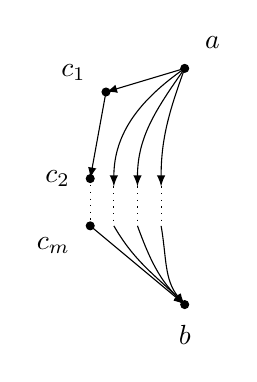
\begin{tikzpicture}
	\draw[arrows={-latex}] (2,2) to [out=250,in=90] (1.7,0.5);
	\draw[arrows={-latex}] (2,2) to [out=235,in=90] (1.4,0.5);
	\draw[arrows={-latex}] (2,2) to [out=215,in=90] (1.1,0.5);
	\draw[fill] (2,2) circle [radius=0.05]
	node [label={[above,xshift=10]$a$}] {};
	\draw[fill] (1,1.7) circle [radius=0.05]
	node [label={[label distance=0.1mm]170:$c_1$}] {};
	\draw[arrows={-latex}] (2,2) -- (1,1.7);
	\draw[fill] (0.8,0.6) circle [radius=0.05]
	node [label={[label distance=0.1mm]180:$c_2$}] {};
	\draw[arrows={-latex}] (1,1.7) -- (0.8,0.6);

	\draw[fill] (0.8,0) circle [radius=0.05]
	node [label={[label distance=0.1mm]190:$c_m$}] {};
	\draw[dotted] (0.8,0.6) -- (0.8,0);
	\draw[dotted] (1.7,0.5) -- (1.7,0);
	\draw[dotted] (1.4,0.5) -- (1.4,0);
	\draw[dotted] (1.1,0.5) -- (1.1,0);

	\draw[fill] (2,-1) circle [radius=0.05]
	node [label={[label distance=0.1mm]270:$b$}] {};
	\draw[arrows={-latex}] (0.8,0) -- (2,-1);
	\draw[arrows={-latex}] (1.7,0) to [out=280,in=130] (2,-1);
	\draw[arrows={-latex}] (1.4,0) to [out=290,in=135] (2,-1);
	\draw[arrows={-latex}] (1.1,0) to [out=300,in=135] (2,-1);
\end{tikzpicture}
	\caption{The trajectories $l_n$ tend to a broken trajectory.}
\end{figure}

Let us consider the general case of a sequence of $\overline{\mathcal{L}}(a,b)$. We can extract a subsequence $(l_n)_n$ such that there are critical points $c_1,...,c_{m-1}$ with $l_n \in \mathcal{L}(a,c_1) \times \cdots \times \mathcal{L}(c_{m-1},b)$. We can do this because the union
\[\overline{\mathcal{L}}(a,b) = \bigcup \mathcal{L}(a,c_1) \times \cdots \times \mathcal{L}(c_{q-1},b)\]
has a finite number of terms, so a infinite number of terms of the sequence $(l_n)_n$ must lie in some of the terms.

Thus, $l_n = (l_n^1,...,l_n^{m-1}) \in \mathcal{L}(a,c_1) \times \cdots \times \mathcal{L}(c_{m-1},b)$. If we apply the previous argument to each of the $(l_n^i)_n$, we can construct a subsequence and a broken trajectory $\mu$ such that $l_n \xrightarrow[n \rightarrow \infty]{} \mu$.
\end{proof}

From here we can start deducing the results that we announced at the beginning of this Section:
\begin{coro}
If $\text{Ind}(a)-\text{Ind}(b) = 1$, the set $\mathcal{L}(a,b)$ is finite.
\end{coro}

\begin{proof}
On one hand, $\text{dim} \mathcal{L}(a,b) = 0$, so it is a discrete set. On the other hand, $\mathcal{L}(a,b) = \overline{\mathcal{L}}(a,b)$, so it is compact. We conclude that it must be finite.
\end{proof}

With this, we have shown that $\partial_X$ is well defined. To prove that $\partial_X^2 = 0$ is more delicate:

\begin{theo} \label{morse_brokenboundary}
If $a, b \in \crit(f)$ and $\text{Ind}(a)-\text{Ind}(b) = 2$, then $\overline{\mathcal{L}}(a,b)$ is a compact manifold with boundary. In addition, the set

\[\bigcup_{c \in \crit(f)} \mathcal{L}(a,c) \times \mathcal{L}(c,b)\]

is the boundary of $\overline{\mathcal{L}}(a,b)$.
\end{theo}

This theorem is proved in Appendix \ref{appendix:brokenboundary}. Assuming that it is true, by the theorem \ref{1dimensional} we have that each connected component of $\overline{\mathcal{L}}(a,b)$ must be diffeomorphic to $\con{S}^1$ or to $[0,1]$. From this, we are able to prove the following result:

\begin{coro} The differential of the Morse complex satisfies that $\partial_X^2 = 0$.
\end{coro}

\begin{proof}
Take $a \in \crit_k(f)$. Then,
\[\partial_X (\partial_X a) = \sum_{b \in \crit_{k-2}(f)} \sum_{c \in \crit_{k-1}(f)} n_X(a,c) n_X(c,b) b =\]
\[= \sum_{b \in \crit_{k-1}(f)} \left( \sum_{c \in \crit_{k-2}(f)} n_X(a,c) n_X(c,b) \right) b .\]
However, we can see that
\[\sum_{c \in \crit_{k-2}(f)} n_X(a,c) n_X(c,b) = \# \left\{ \bigcup_{c \in \crit(f)} \mathcal{L}(a,c) \times \mathcal{L}(c,b) \right\} \quad (\text{mod } 2).\]

As we just said, the term on the right is the boundary of a 1-dimensional compact manifold with boundary (not necessarily connected), so it has an even number of points. Therefore, its cardinal modulo 2 must be 0.
\end{proof}
